\documentclass[twoside]{article}
\usepackage[utf8]{inputenc}
\usepackage[T1]{fontenc}
\usepackage{graphicx, xcolor}
\usepackage{latexsym, amsthm, amsfonts, amsmath, amscd, eucal, amssymb, epsf, mathtools, bbm}
\usepackage{tikz}
\usetikzlibrary{patterns}
\usepackage{pgfplots}

\begin{document}

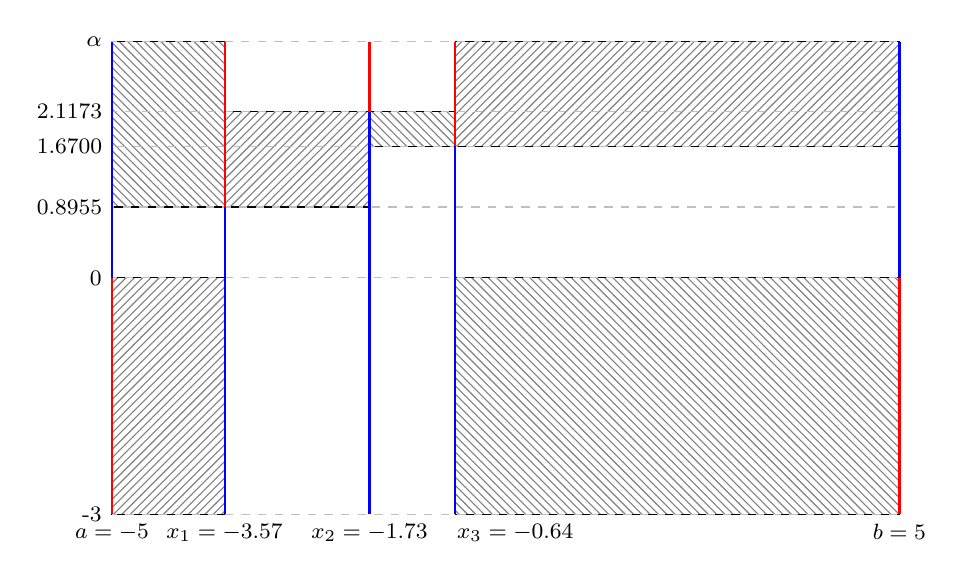
\begin{tikzpicture}

\draw[pattern=north west lines, pattern color=black!50] (-5, 0.90) node[anchor=east]{\footnotesize{0.8955}} rectangle  (-3.57, 3);
\draw[pattern=north east lines, pattern color=black!50] (-3.57, 0.90) rectangle  (-1.73, 2.11);
\draw[pattern=north west lines, pattern color=black!50] (-1.73, 2.11) rectangle  (-0.64, 1.67);
\draw[pattern=north east lines, pattern color=black!50] (-0.64, 1.67) rectangle  (5, 3);
\draw[pattern=north east lines, pattern color=black!50] (-5, -3) rectangle  (-3.57, 0);
\draw[pattern=north west lines, pattern color=black!50] (-0.64, -3) rectangle  (5, 0);
\draw [dashed, black!25] (-5, -3) rectangle  (5, 0);
\draw [dashed, black!25] (-5, 0.90) rectangle  (5, 1.67);
\draw [dashed, black!25] (-5, 2.11) node[anchor=east, black]{\footnotesize{2.1173}} rectangle  (5, 3);
\draw[thick, red](-5, -3) node[anchor=east, black]{\footnotesize{-3}}  -- (-5, 0);
\draw[thick, blue](-5, 0) node[anchor=east, black]{\footnotesize{0}} -- (-5, 3) node[anchor=east, black]{\footnotesize{$\alpha$}};
\draw[thick, red](5, -3) -- (5, 0);
\draw[thick, blue](5, 0) -- (5, 3);
\draw[thick, blue](-3.57, -3) -- (-3.57, 0.90);
\draw[thick, red](-3.57, 0.90) -- (-3.57, 3);
\draw[thick, blue](-1.73, -3) -- (-1.73, 2.11);
\draw[thick, red](-1.73, 2.11) -- (-1.73, 3);
\draw[thick, blue](-0.64, -3) -- (-0.64, 1.67);
\draw[thick, red](-0.64, 1.67) -- (-0.64, 3);
\node[anchor=east, black] at (-5, 1.67){\footnotesize{1.6700}};
\node[anchor= north, black] at (-5, -3){\footnotesize{$a = -5$}};
\node[anchor= north, black] at (5, -3){\footnotesize{$b = 5$}};
\node[anchor= north, black] at (-3.57, -3){\footnotesize{$x_1 = -3.57$}};
\node[anchor= north, black] at (-1.73, -3){\footnotesize{$x_2 = -1.73$}};
\node[anchor= north west, black] at (-0.74, -3){\footnotesize{$x_3 = -0.64$}};

\end{tikzpicture}

\end{document}